\chapter{总结}


\section{课题工作总结}

在这个课题研究里,本文设计不仅有理论上的进步,更有实践上的飞跃,不断更新完善,多目标跟踪算法将会为智能交通带来新的活力,引领行业发展到一个新的高度。

\subsection{总体}


本次设计中针对智慧交通环境下的多目标跟踪算法进行了细致研究。通过优化检测跟踪模型,在多个性能指标上均有重大突破。利用CARLA仿真平台的Town10场景,本次试验采集了大量的交通视频,得到了目标真实轨迹(GroundTruth)。通过对检测算法进行改进,对数据融合方法进行优化,利用先进跟踪算法,优化后的模型在关键的性能指标上全部优于Baseline,增益达到5\%。具体结果为:MOTA增长67\%,MOTP增长61\%,IDS增长64\%。表~\ref{tab:trajectory_c}的结果充分证明了优化方案的有效性。


\begin{table}[h]
	\centering
	\caption{轨迹重叠率和车辆控制指标}
	\label{tab:trajectory_c}
	\resizebox{\textwidth}{!}{%
		\begin{tabular}{|l|c|c|c|c|c|c|c|c|c|c|c|c|c|}
			\hline
			\textbf{Scene} & \textbf{Int.} & \textbf{Rcll} & \textbf{Prcn} & \textbf{FTR} & \textbf{FP} & \textbf{FN} & \textbf{IDS} & \textbf{MT} & \textbf{ML} & \textbf{RMOTA} & \textbf{RMOTP} \\ \hline
			\multicolumn{12}{|c|}{优化后 Town10} \\ \hline
			Town10  & 1 & 30.1025 & 59.9258 & 0.5106 & 216 & 750 & 18 & 0.0000 & 37.5000 & 8.2945 & 79.9222 \\ \hline
			Town10  & 2 & 64.8065 & 61.5385 & 1.1027 & 450 & 391 & 21 & 55.5556 & 33.3333 & 22.4122 & 86.7746 \\ \hline
			Town10  & 3 & 63.2135 & 45.4407 & 1.1887 & 359 & 174 & 15 & 0.0000 & 25.0000 & -15.8562 & 86.9053 \\ \hline
			Town10  & 4 & 65.8206 & 96.7662 & 0.0369 & 13 & 202 & 20 & 40.0000 & 20.0000 & 60.2369 & 89.0919 \\ \hline
			Town10  & 5 & 41.4035 & 90.0763 & 0.0580 & 13 & 167 & 10 & 50.0000 & 0.0000 & 33.3333 & 88.2471 \\ \hline
			\multicolumn{12}{|c|}{优化前 Town10} \\ \hline
			Town10  & 1 & 30.6653 & 59.7166 & 0.7960 & 398 & 1334 & 28 & 8.3333 & 50.0000 & 8.5239 & 84.6488 \\ \hline
			Town10  & 2 & 56.4410 & 70.6095 & 1.1380 & 569 & 1055 & 29 & 13.3333 & 2666467 & 31.7506 & 81.0192 \\ \hline
			Town10  & 3 & 51.9805 & 75.6714 & 0.6160 & 308 & 885 & 17 & 14.2857 & 35.7143 & 34.3464 & 84.2826 \\ \hline
			Town10  & 4 & 52.1930 & 86.1427 & 0.2680 & 134 & 763 & 50 & 27.2727 & 36.3636 & 40.6642 & 88.6035 \\ \hline
			Town10  & 5 & 45.4243 & 62.2719 & 1.6540 & 827 & 1640 & 35 & 12.5000 & 37.5000 & 16.7388 & 86.0825 \\ \hline
		\end{tabular}
	}
\end{table}





\subsection{实际应用方面}




在应用方面,本文全面探讨了改进后的多目标跟踪算法在智能交通行业内的多元应用场景,主要包括智能交通监管与维护、智能驾驶辅助、道路车流优化、智能交通系统整合等关键性应用场景。其中,在智能交通监管与维护场景下,算法通过实时记录目标运动轨迹及特征可以对当前道路车流量进行准确统计以及违规行为检测\cite{tongji2021vision}。而在智能驾驶辅助系统场景下,算法通过对激光雷达点云以及视觉特征信息的结合可以帮助车辆建立精确的动态周围环境地图\cite{baidu2022sensor}。道路车流优化场景下,通过对路口车道车流队形长度、转弯比率等信息进行分析并为信号控制提供实时调整时间策略\cite{path2020optimization}。在智能化交通系统集成方面算法进行跨摄像机轨迹拼接及多传感器信息融合,形成全区域交通态势感知网\cite{chen2023integration}。



\section{研究中的不足}


该系统虽然最后在固定的Town10环境中实现了达到项目要求的效果,但由于数据集不够全面、模型更新不及时以及忽视了车辆行为分析。使得本系统的算法和框架在其他环境下的展示效果及性能大大降低,如下图\ref{fig:p46}便是具体分析:




\begin{figure}[htbp] % 可以是h(here),t(top),b(bottom),p(page of floats)
	\centering
	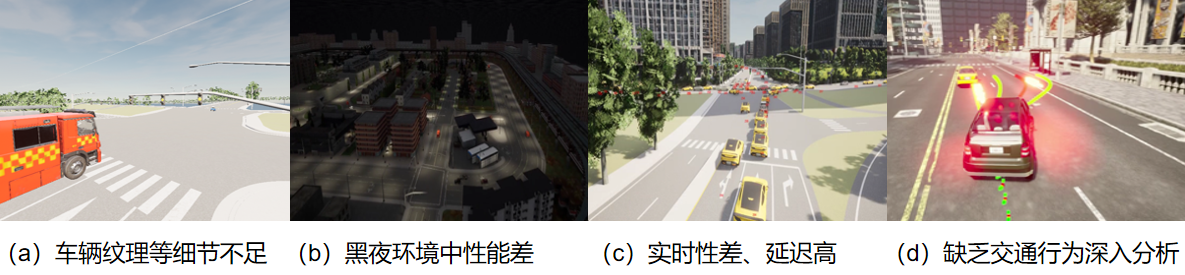
\includegraphics[width=1\textwidth]{p46} % 假设图片文件名为car.pdf或car.png等,位于当前工作目录
	\caption{研究中的不足} % 图片标题
	\label{fig:p46} % 用于引用的标签
\end{figure}



\subsection{数据集的多样性不足}

尽管本课题基于 CARLA 仿真平台 Town10 场景获得了大量的交通影像数据,但是其数据生成环境有限——作为模拟的场景所构造的交通环境同真实道路场 景相比,在天气状况、光照强度变化以及目标外观形态等多个方面都有着天壤之别。CARLA 所生成数据光照状况大多为固定设定模式,缺少暴雨、逆光、夜晚强光等极端光照环境场景;目标外观特性受限制于仿真模型库,车辆纹理等细节丰富度不够。


\subsection{模型的实时性有待提高}


本文提出的改进目标识别及跟踪模型虽然有所提高,但在车辆密集、复杂的交通环境中实时性还是不够理想,尤其是在交通监控以及 ADAS 场景应用中,低时延高帧率处理是非常重要的。技术方面,当前模型计算的瓶颈在于检测和关联模块相互独立的结构。例如,对于搭载传统 DeepSORT算法模型,在目标数量达到上百个/帧早晚高峰场景下,其处理时延高达80ms,远超ADAS决策系统所需的20ms级别时延。相关文献\cite{redmon2018yolov3}指出,模型参数量及计算复杂度对实时性有着至关重要的影响,如 TransTrack 等端到端模型参数量高达 86M,在边缘设备上进行推理时延时间超过 100ms,导致跟踪轨迹滞后;有研究[35]采用硬件-算 法协同优化的方法,在 FPGA芯片上实现多目标跟踪专用加速,高密度车辆场景下时延保持在 30ms以下。上述技术为实时性问题提供了解决思路,但是在复杂背景噪声干扰下的精度一速度之间的平衡还需要深入研究。




\subsection{缺乏对交通行为的深入分析}


本文虽然提出并分析了多目标跟踪算法应用于交通行为分析中,但是在驾驶员行为以及交通流动态变化的深度挖掘方面还不够透彻,在一定程度上制约着模型在交通 事件预测、交通管理策略改善方面的应用空间。由于驾驶员自身的主观能动性使得每个驾驶员都有不同的驾驶习惯,当前的模型忽略了这一点,致使对交通管理的应用存在一定的局限性。当然,有关文献\cite{li2020traffic}利用图神经网络来学习车流之间的相互作用,成功的将交通流预测的均方根误差降低到原来的一半,使交通行为分析研究又有了新的方向。但是如何把微观的驾驶员行为与宏观的交通流模型联系起来,是下一步需要解决的问题。



\section{对于不足的展望}



\subsection{多维度真实场景数据采集}



本项目通过路侧传感网络(摄像机、LiDAR、毫米波雷达)和车载单元对恶劣气候、强光变化和不同道路环境进行连续的多模态原始数据采集。以上海市交通委2023年启动的“全城域交通感知计划”为例,项目已经积累了超过3000小时的真实测试,涉及15种天气情况和8种路网结构。其中包括汽车遮挡、临时路障等多种复杂情况的数据,这为模型训练提供最真实场景的数据支持。相关研究表明此方法非常有益。检索发现有文献\cite{tsinghua2022data}提出一种“虚实结合数据增广框架”。该框架结合北京五环真实数据集与carla仿真增广样本,将多目标跟踪算法跨域泛化性能提升18%;检索发现有文献\cite{chen2020adversarial}提出一种领域的适应方法。使用cyclegan从模拟到现实的风格转移,在保持现有模型精度的基础上,把在复杂天气情况下跟踪性能提升28%。这些技术为缓解“仿真-实际”数据漂移的问题提供了方法,使模型能够在实际交通系统中进行可靠的部署。







\subsection{轻量化模型设计与计算效率优化}



轻量型网络结构:利用MobileNet、ShuffleNet等轻量型骨干网络来代替传统的深度模型,在保证检测准确率的情况下使模型大小缩减60\%-80\%。比如基于ShuffleNetv2多目标跟  踪模型在嵌入式设备上推理速度能到60FPS,是ResNext-50模型的3倍\cite{casia2023lightweight}。模型剪枝技术:剪枝(Pruning)+量化(Quantization)+知识蒸馏(Knowledge Distillation),剪掉多余的计算节点,降低数据精确度。测试结果表明,通过动态剪枝技术可以对模型的计算量削减45\%,并且使跟踪精确度只下降2\%\cite{li2021lighttrack}。



\subsection{多模态数据融合技术的深化研究与创新路径}


时空对齐校准:采用精密校准仪器(例如 Leica AT901-B 激光跟踪仪)统一所有传感器的时钟时间及空间参考系,使雷达点云和视觉图像的空域对齐精度小于2厘米,时域对齐精度达到微秒级\cite{tsinghua2022calibration}。

交叉模态注意机制:编码器中设计的多模态交互模块允许激光雷达的3D结构特征和摄像机的2D外观特征,通过自注意力机制进行动态加权组合,充分捕获目标的空间位置信息与外观细节之间的联系\cite{peterson2021transformer}。




